% Tidal-Induced Stellar Warp Paper
% Format: MNRAS (Monthly Notices of the Royal Astronomical Society)
\documentclass[fleqn,usenatbib]{mnras}

\usepackage{newtxtext,newtxmath}
\usepackage{graphicx}
\usepackage{amsmath,amssymb}
\usepackage{booktabs}
\usepackage{multirow}
\usepackage{hyperref}
\usepackage{xcolor}

% Title
\title[Tidal-Induced Stellar Warps]{Impulsive tidal excitation of stellar disk warps: \\
a tilted-ring model study}

\author[Author et al.]{
Author One,$^{1}$\thanks{E-mail: author@university.edu}
Author Two$^{1}$
and Author Three$^{2}$
\\
$^{1}$Department of Astronomy, University, City, Country\\
$^{2}$Institute for Advanced Study, City, Country
}

\date{Accepted XXX. Received YYY; in original form ZZZ}

\pubyear{2026}

\begin{document}

\label{firstpage}
\pagerange{\pageref{firstpage}--\pageref{lastpage}}
\maketitle

% ============================================================
% ABSTRACT
% ============================================================
\begin{abstract}
Galactic disk warps are ubiquitous in spiral galaxies, yet the dominant mechanism responsible for their excitation remains debated. We investigate the tidal origin of stellar warps using a tilted-ring dynamical model in which the disk is decomposed into 60 concentric rings evolving under three torques: disk self-gravity coupling, an oblate NFW dark matter halo, and the quadrupole tidal field of an orbiting satellite galaxy. Integration is performed with a fourth-order Runge--Kutta scheme over 3\,Gyr.

Our fiducial model (satellite mass $M_\mathrm{sat}=10^{11}\,\mathrm{M}_\odot$, semi-major axis $a=25$\,kpc, eccentricity $e=0.3$, orbital inclination $i=45^\circ$) produces a peak warp tilt of $1.70^\circ$, with an outer-disk ($R>10$\,kpc) tilt of $1.34^\circ$. The warp grows in a characteristic \emph{staircase pattern}, with each step synchronized to a pericentric passage of the satellite, demonstrating that warp growth is impulsive rather than continuous. The line of nodes precesses coherently at ${\sim}7\,\mathrm{deg\,Gyr}^{-1}$, consistent with recent \textit{Gaia}-based measurements.

A parameter study reveals that warp amplitude scales linearly with satellite mass, peaks at orbital inclination $i\approx45^\circ$ following a $\sin 2i$ dependence, and is insensitive to halo flattening when a strong tidal perturber is present. Torque decomposition shows that the tidal torque dominates over disk self-gravity by 1--3 orders of magnitude at $R>2$\,kpc, while the halo torque is subdominant by ${\sim}3$ orders of magnitude. The model reproduces the qualitative features of the Milky Way warp, including the radially increasing tilt profile and the absence of strong winding, though the predicted amplitude lies at the lower end of observational estimates, likely due to the omission of the dynamical halo response.
\end{abstract}

\begin{keywords}
galaxies: kinematics and dynamics -- galaxies: structure -- Galaxy: disc -- Galaxy: evolution -- methods: numerical
\end{keywords}

% ============================================================
% 1. INTRODUCTION
% ============================================================
\section{Introduction}
\label{sec:intro}

Warps -- large-scale bending of the outer disk out of the galactic midplane -- are among the most common structural features of spiral galaxies. Observations in neutral hydrogen (\ion{H}{i}) have long established that the majority of disk galaxies exhibit warped gas layers \citep{garciaruiz2002, kruit2007}, and the phenomenon extends to the stellar component as revealed by infrared photometry and, more recently, by precision astrometry from \textit{Gaia} \citep{poggio2020, chen2019, skowron2019}.

The Milky Way itself hosts a prominent warp. Classical Cepheid mapping by \citet{chen2019} and \citet{skowron2019} reveals a stellar warp reaching a physical displacement of ${\sim}0.5$--$1.0$\,kpc at $R\sim14$\,kpc, corresponding to a tilt angle of ${\sim}2^\circ$--$5^\circ$ depending on the tracer population and the radial range considered. The \ion{H}{i} gas warp extends further, reaching displacements of ${\sim}3$--$4$\,kpc at $R\sim25$\,kpc \citep{bland2016}. Recent kinematic analyses using \textit{Gaia} data have additionally detected the warp's time evolution: the line of nodes precesses at a rate of ${\sim}10$--$13\,\mathrm{km\,s^{-1}\,kpc^{-1}}$ (equivalently ${\sim}5$--$10\,\mathrm{deg\,Gyr^{-1}}$), a measurement that constrains the underlying dynamics \citep{poggio2020, cheng2020}.

Despite the ubiquity of galactic warps, the dominant excitation mechanism remains a matter of active debate \citep[see][for reviews]{binney1992, bland2016}. The principal hypotheses include:

\begin{enumerate}
    \item \textbf{Tidal interaction with satellite galaxies.} A companion galaxy on an inclined orbit exerts a time-varying quadrupole tidal torque that can tilt the outer disk differentially \citep{hunter1969, ostriker1989, weinberg1998, tsuchiya2002}. In the Milky Way context, both the Large Magellanic Cloud (LMC; $M\sim1$--$2\times10^{11}\,\mathrm{M}_\odot$; \citealt{erkal2019}) and the Sagittarius dwarf galaxy \citep{laporte2018, bennett2022} have been proposed as drivers.
    
    \item \textbf{Misaligned dark matter halo.} If the disk angular momentum is misaligned with the principal axes of an oblate or triaxial dark matter halo, the resulting torque drives differential precession of disk annuli, which can manifest as a warp \citep{debattista1999, sparke1988}.
    
    \item \textbf{Cosmic gas accretion.} Misaligned infall of intergalactic gas onto the outer disk can torque the disk directly \citep{lopezcorredoira2002}.
    
    \item \textbf{Internally driven bending waves.} Any perturbation that misaligns the inner and outer disk excites a retrograde bending wave that propagates outward and grows in amplitude \citep{sellwood2022}.
\end{enumerate}

These mechanisms are not mutually exclusive, and the observed warp in any given galaxy likely reflects a combination of drivers. Nevertheless, identifying the \emph{dominant} mechanism is crucial for using warps as probes of galactic dynamics and dark matter halo properties.

In this work, we focus on the tidal mechanism and investigate its consequences using a tilted-ring dynamical model. The tilted-ring approach, pioneered by \citet{sparke1988}, decomposes the disk into concentric rings whose angular momentum vectors evolve under mutual gravitational torques, halo torques, and external forcing. This semi-analytic framework captures the essential physics of warp excitation and propagation -- including self-gravity mediated bending stiffness, differential precession, and tidal driving -- while being computationally efficient enough to permit extensive parameter surveys.

Our study makes three principal contributions:
\begin{enumerate}
    \item We demonstrate that tidal warp growth is \emph{impulsive}: the warp amplitude increases in discrete steps synchronized with the satellite's pericentric passages, rather than growing continuously (Section~\ref{sec:fiducial}).
    \item We quantify the scaling of warp amplitude with satellite mass (${\propto}M_\mathrm{sat}$), orbital inclination (${\propto}\sin 2i$), and halo flattening, providing analytic understanding for each dependence (Section~\ref{sec:params}).
    \item We decompose the torque budget as a function of galactocentric radius, revealing that tidal torques dominate over disk self-gravity by 1--3 orders of magnitude at $R>2$\,kpc, while the halo torque is subdominant by ${\sim}3$ orders of magnitude (Section~\ref{sec:torques}).
\end{enumerate}

The paper is organized as follows. Section~\ref{sec:method} describes the tilted-ring model, the galactic potential, the satellite orbit, and the numerical integration scheme. Section~\ref{sec:results} presents the results of the fiducial simulation and the parameter study. Section~\ref{sec:discussion} compares with observations and discusses caveats. Section~\ref{sec:conclusions} summarizes our conclusions.


% ============================================================
% 2. METHOD
% ============================================================
\section{Method}
\label{sec:method}

\subsection{Tilted-ring model}
\label{sec:ring_model}

We model the stellar disk as a collection of $N=60$ concentric, infinitesimally thin rings spanning radii $R_\mathrm{min}=0.5$\,kpc to $R_\mathrm{max}=18$\,kpc with uniform spacing $\Delta R = (R_\mathrm{max}-R_\mathrm{min})/N \approx 0.29$\,kpc. Each ring $i$ is characterized by its radius $R_i$, mass $M_i$, and angular momentum unit vector $\hat{\boldsymbol{L}}_i(t)$. The direction of $\hat{\boldsymbol{L}}_i$ encodes the instantaneous tilt of ring $i$ relative to the reference plane ($z$-axis).

The ring masses are assigned assuming an exponential surface density profile:
\begin{equation}
    \Sigma(R) = \frac{M_\mathrm{disk}}{2\pi R_d^2} \exp\!\left(-\frac{R}{R_d}\right),
\end{equation}
where $M_\mathrm{disk}=5\times10^{10}\,\mathrm{M}_\odot$ is the total disk mass and $R_d=3.5$\,kpc is the exponential scale length. The mass of ring $i$ is then $M_i = 2\pi R_i \,\Sigma(R_i)\,\Delta R$.

Each ring's circular velocity is computed from the enclosed mass of the combined NFW halo and exponential disk:
\begin{equation}
    v_\mathrm{circ}(R) = \sqrt{\frac{G\left[M_\mathrm{enc}^\mathrm{halo}(R) + M_\mathrm{enc}^\mathrm{disk}(R)\right]}{R}},
\end{equation}
where $M_\mathrm{enc}^\mathrm{disk}(R) = M_\mathrm{disk}\left[1-(1+R/R_d)\exp(-R/R_d)\right]$ and the NFW enclosed mass is given in Section~\ref{sec:halo}. The angular velocity is $\Omega_i = v_\mathrm{circ}(R_i)/R_i$ and the specific angular momentum is $\ell_i = v_\mathrm{circ}(R_i)\,R_i$.

\subsection{Dark matter halo}
\label{sec:halo}

The host galaxy's dark matter halo is modeled as a Navarro--Frenk--White \citep[NFW;][]{navarro1996} profile with virial mass $M_\mathrm{vir}=10^{12}\,\mathrm{M}_\odot$, concentration $c=12$, and virial radius $R_\mathrm{vir}=200$\,kpc. The enclosed mass is
\begin{equation}
    M_\mathrm{enc}^\mathrm{halo}(r) = \frac{M_\mathrm{vir}}{\ln(1+c) - c/(1+c)} \left[\ln(1+x) - \frac{x}{1+x}\right],
\end{equation}
where $x = r/R_s$ and $R_s = R_\mathrm{vir}/c$ is the scale radius.

To model the effect of a slightly oblate halo, we introduce the axis ratio $q \leq 1$, parameterizing the halo flattening. The oblateness produces a torque on tilted rings that causes differential precession. The precession frequency is
\begin{equation}
    \nu_p^2(R) = (1-q^2)\,\frac{G\,M_\mathrm{enc}^\mathrm{halo}(R)}{R^3}.
    \label{eq:nu_p}
\end{equation}
Our fiducial model adopts $q=0.95$, corresponding to a mildly oblate halo.

\subsection{Torques}
\label{sec:torques_method}

The evolution of each ring's angular momentum direction is governed by
\begin{equation}
    \frac{\mathrm{d}\hat{\boldsymbol{L}}_i}{\mathrm{d}t} = \frac{\boldsymbol{T}_i^\mathrm{self} + \boldsymbol{T}_i^\mathrm{halo} + \boldsymbol{T}_i^\mathrm{tidal}}{M_i\,\ell_i},
    \label{eq:dLdt}
\end{equation}
where $M_i\,\ell_i = |\boldsymbol{L}_i|$ is the angular momentum magnitude, and the three torque terms are described below.

\subsubsection{Self-gravity coupling}

When neighboring rings are mutually tilted, they exert gravitational torques on each other that resist differential bending. Following \citet{sparke1988}, the coupling torque on ring $i$ from ring $j$ is
\begin{equation}
    \boldsymbol{T}_{ij}^\mathrm{self} = C_{ij}\,\hat{\boldsymbol{L}}_i \times \left(\hat{\boldsymbol{L}}_j \times \hat{\boldsymbol{L}}_i\right),
\end{equation}
where the coupling coefficient is
\begin{equation}
    C_{ij} = \frac{G\,M_i\,M_j\,\min(R_i,R_j)}{r_\mathrm{eff}^2\,\max(R_i,R_j)},
\end{equation}
and $r_\mathrm{eff} = \sqrt{|R_i-R_j|^2 + h^2}$ is the effective separation softened by the disk scale height $h=z_\mathrm{disk}=0.3$\,kpc. The total self-gravity torque on ring $i$ is $\boldsymbol{T}_i^\mathrm{self}=\sum_{j\neq i} \boldsymbol{T}_{ij}^\mathrm{self}$, summed over the nearest 8 neighbors in each direction.

This coupling provides the disk's \emph{bending stiffness}: it resists differential tilting and enables the propagation of bending waves through the disk.

\subsubsection{Halo torque}

The oblate halo exerts a torque that drives precession of tilted rings around the halo symmetry axis ($\hat{\boldsymbol{z}}$):
\begin{equation}
    \boldsymbol{T}_i^\mathrm{halo} = \nu_p^2(R_i)\,M_i\,\ell_i\,\left(\hat{\boldsymbol{z}} \times \hat{\boldsymbol{L}}_i\right),
    \label{eq:T_halo}
\end{equation}
where $\nu_p^2$ is given by equation~(\ref{eq:nu_p}). This torque is perpendicular to both $\hat{\boldsymbol{z}}$ and $\hat{\boldsymbol{L}}_i$, causing pure precession without changing the tilt angle.

\subsubsection{Tidal torque}
\label{sec:tidal_torque}

The satellite galaxy, treated as a point mass $M_\mathrm{sat}$ at position $\boldsymbol{r}_\mathrm{sat}(t)$, exerts a quadrupole tidal torque on each ring:
\begin{equation}
    \boldsymbol{T}_i^\mathrm{tidal} = \frac{3}{2}\,\frac{G\,M_\mathrm{sat}\,M_i\,R_i^2}{d^3}\,\left(\hat{\boldsymbol{d}} \times \hat{\boldsymbol{L}}_i\right)\left(\hat{\boldsymbol{d}} \cdot \hat{\boldsymbol{L}}_i\right),
    \label{eq:T_tidal}
\end{equation}
where $d = |\boldsymbol{r}_\mathrm{sat}|$ is the distance from the galactic centre to the satellite (softened by $\epsilon_\mathrm{sat}$) and $\hat{\boldsymbol{d}} = \boldsymbol{r}_\mathrm{sat}/d$. The key features of this torque are:
\begin{itemize}
    \item It scales as $R_i^2/d^3$, making the outer disk far more susceptible than the inner disk.
    \item The factor $(\hat{\boldsymbol{d}}\cdot\hat{\boldsymbol{L}}_i)(\hat{\boldsymbol{d}}\times\hat{\boldsymbol{L}}_i)$ vanishes when the satellite is in the disk plane ($\hat{\boldsymbol{d}}\perp\hat{\boldsymbol{L}}_i$) or along the disk normal ($\hat{\boldsymbol{d}}\parallel\hat{\boldsymbol{L}}_i$), and is maximized at an angle of $45^\circ$ between the two vectors.
\end{itemize}

\subsection{Satellite orbit}
\label{sec:orbit}

The satellite follows a fixed Keplerian orbit with semi-major axis $a$, eccentricity $e$, and inclination $i$ relative to the disk plane. The orbital position is obtained by solving Kepler's equation iteratively at each time-step. The pericentric distance is $d_\mathrm{peri} = a(1-e)$ and the orbital period is $P$.

Table~\ref{tab:params} summarizes the fiducial model parameters.

\begin{table}
    \centering
    \caption{Fiducial model parameters.}
    \label{tab:params}
    \begin{tabular}{lcc}
        \toprule
        Parameter & Symbol & Value \\
        \midrule
        \multicolumn{3}{l}{\textit{Stellar disk}} \\
        Total mass & $M_\mathrm{disk}$ & $5\times10^{10}\,\mathrm{M}_\odot$ \\
        Scale length & $R_d$ & 3.5\,kpc \\
        Scale height & $h$ & 0.3\,kpc \\
        Number of rings & $N$ & 60 \\
        Radial range & $R$ & 0.5--18\,kpc \\
        \midrule
        \multicolumn{3}{l}{\textit{NFW dark matter halo}} \\
        Virial mass & $M_\mathrm{vir}$ & $10^{12}\,\mathrm{M}_\odot$ \\
        Concentration & $c$ & 12 \\
        Virial radius & $R_\mathrm{vir}$ & 200\,kpc \\
        Axis ratio & $q$ & 0.95 \\
        \midrule
        \multicolumn{3}{l}{\textit{Satellite galaxy}} \\
        Mass & $M_\mathrm{sat}$ & $10^{11}\,\mathrm{M}_\odot$ \\
        Semi-major axis & $a$ & 25\,kpc \\
        Eccentricity & $e$ & 0.3 \\
        Orbital inclination & $i$ & $45^\circ$ \\
        Orbital period & $P$ & 800\,Myr \\
        Softening length & $\epsilon_\mathrm{sat}$ & 2\,kpc \\
        \midrule
        \multicolumn{3}{l}{\textit{Numerical}} \\
        Time-step & $\Delta t$ & 1\,Myr \\
        Total time & $T$ & 3000\,Myr \\
        Snapshot interval & & 25\,Myr \\
        \bottomrule
    \end{tabular}
\end{table}

\subsection{Numerical integration}
\label{sec:integration}

The system of ordinary differential equations~(\ref{eq:dLdt}) is integrated using a fourth-order Runge--Kutta (RK4) scheme with a fixed time-step $\Delta t = 1$\,Myr. After each full RK4 step, the unit vectors $\hat{\boldsymbol{L}}_i$ are renormalized to maintain $|\hat{\boldsymbol{L}}_i|=1$.

We adopt a unit system in which lengths are in kpc, masses in $10^{10}\,\mathrm{M}_\odot$, and times in Myr. The gravitational constant in these units is $G = 4.498\times10^{-6}\,\mathrm{kpc}^3/(10^{10}\,\mathrm{M}_\odot\,\mathrm{Myr}^2)$.

The total integration time is $T=3000$\,Myr, corresponding to approximately 3.75 orbital periods of the satellite. Snapshots of $\hat{\boldsymbol{L}}_i(t)$ are saved every 25\,Myr for post-processing.

\subsection{Diagnostics}
\label{sec:diagnostics}

We characterize the warp through two primary diagnostics:

\begin{enumerate}
    \item \textbf{Tilt angle} $\theta_i(t) = \arccos(\hat{L}_{i,z})$: the angle between ring $i$'s angular momentum vector and the $z$-axis. A flat disk has $\theta_i=0$ for all $i$.
    
    \item \textbf{Line of nodes} $\phi_i(t) = \arctan(\hat{L}_{i,y}/\hat{L}_{i,x})$: the azimuthal direction of ring $i$'s tilt. A coherent warp has $\phi_i \approx \mathrm{const}$ across all radii; a wound-up warp shows $\phi_i$ varying strongly with $R$.
\end{enumerate}

We also report the maximum tilt angle across all rings, $\theta_\mathrm{max}(t) = \max_i \theta_i(t)$, and the mean tilt of the outer disk, $\langle\theta\rangle_\mathrm{outer}(t) = \langle\theta_i\rangle_{R_i>10\,\mathrm{kpc}}$.


% ============================================================
% 3. RESULTS
% ============================================================
\section{Results}
\label{sec:results}

\subsection{Baseline: isolated disk}
\label{sec:baseline}

We first verify that the model produces a stable, flat disk in the absence of tidal perturbation. Running the baseline simulation ($M_\mathrm{sat}=0$) for 3\,Gyr, we find that all rings maintain $\theta_i < 10^{-10}\,\mathrm{deg}$ throughout the integration. This confirms that the numerical scheme preserves the equilibrium state and that any warp detected in the tidal simulations is a genuine response to the satellite forcing.

\subsection{Fiducial tidal simulation}
\label{sec:fiducial}

Fig.~\ref{fig:warp_evolution} presents the fiducial simulation results ($M_\mathrm{sat}=10^{11}\,\mathrm{M}_\odot$, $i=45^\circ$, $e=0.3$).

\begin{figure*}
    \centering
    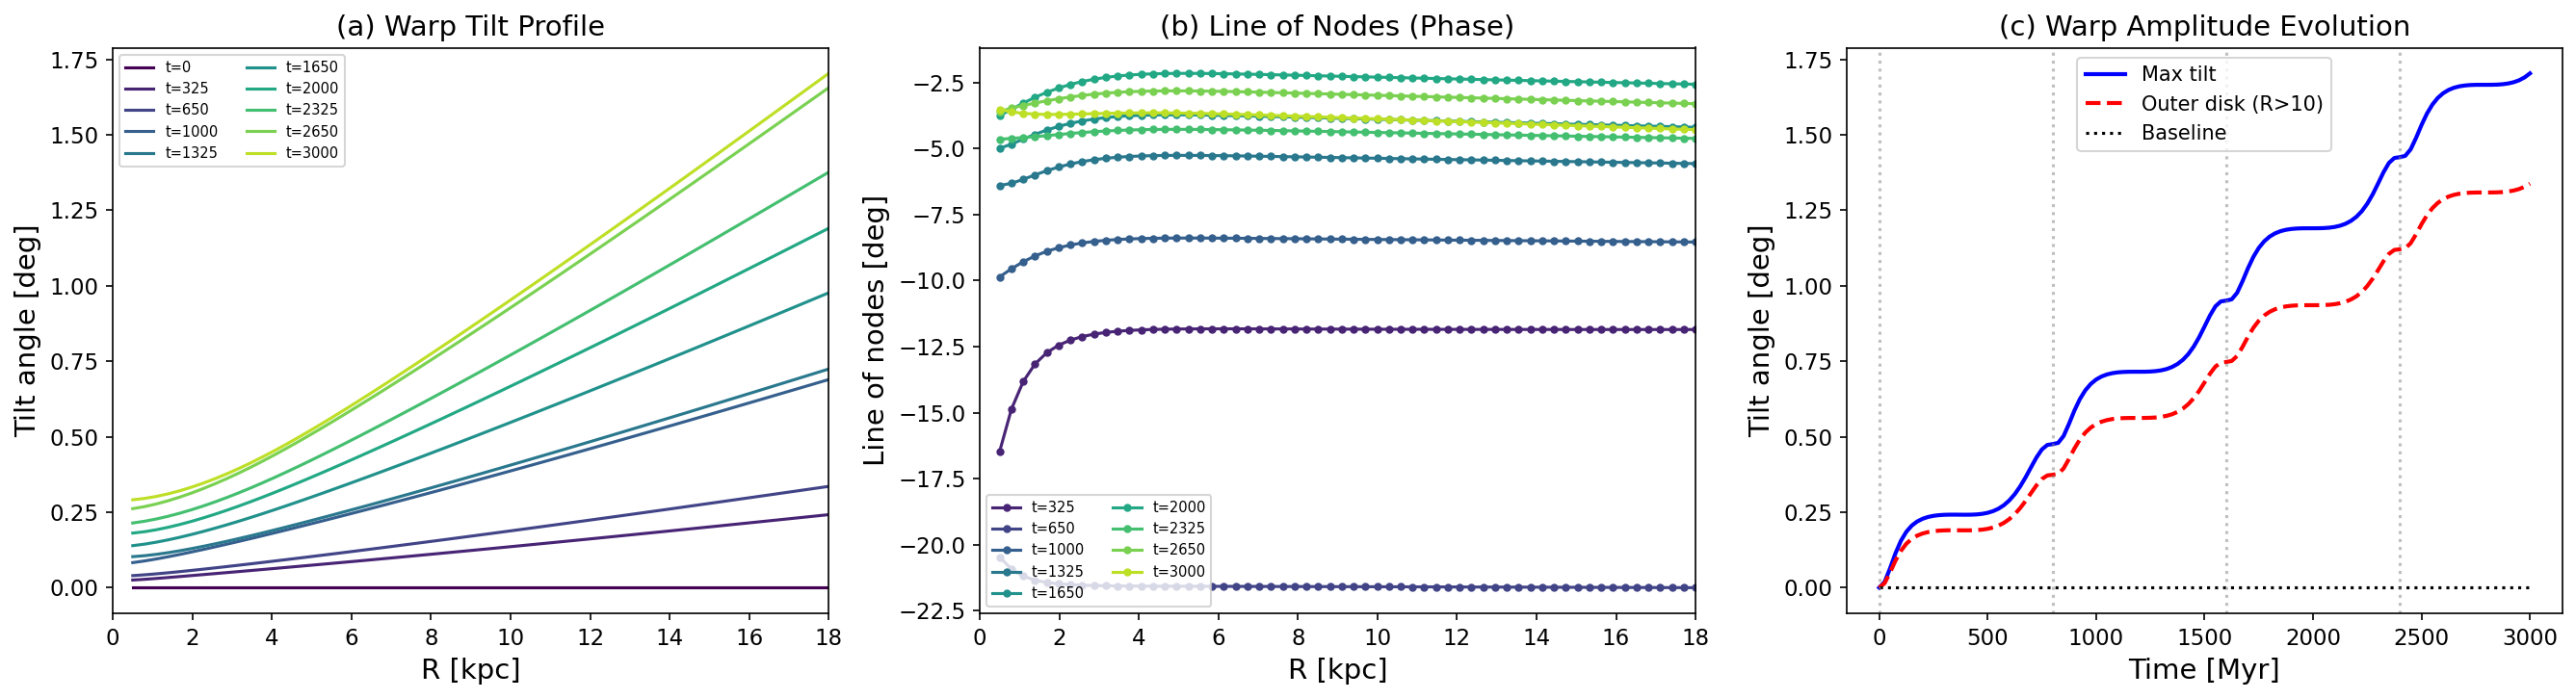
\includegraphics[width=\textwidth]{fig1_warp_evolution.png}
    \caption{Evolution of the stellar warp in the fiducial tidal simulation. \textbf{(a)} Warp tilt profile $\theta(R)$ at selected times (colour-coded). The tilt grows monotonically with radius, confirming that the outer disk is most susceptible to tidal torquing. \textbf{(b)} Line of nodes $\phi(R)$ at the same times, showing coherent precession (near-constant $\phi$ with $R$). \textbf{(c)} Time evolution of the maximum tilt (blue solid) and the mean outer-disk tilt for $R>10$\,kpc (red dashed). Vertical dotted lines mark pericentric passages ($P=800$\,Myr). The baseline (black dotted) remains flat. Note the characteristic \emph{staircase} growth pattern.}
    \label{fig:warp_evolution}
\end{figure*}

\subsubsection{Radial tilt profile}

Panel~(a) of Fig.~\ref{fig:warp_evolution} shows the tilt angle as a function of radius at ten epochs spanning $t=0$--$3000$\,Myr. Several features are noteworthy:
\begin{itemize}
    \item The tilt increases monotonically with radius at all times, consistent with the $R^2$ scaling of the tidal torque (equation~\ref{eq:T_tidal}).
    \item The inner disk ($R\lesssim4$\,kpc) remains nearly flat ($\theta < 0.1^\circ$ even at $t=3$\,Gyr), stabilized by the disk's bending stiffness provided by self-gravity coupling.
    \item At the final time, the maximum tilt is $\theta_\mathrm{max}=1.70^\circ$ at $R=18$\,kpc, and the mean outer-disk ($R>10$\,kpc) tilt is $\langle\theta\rangle_\mathrm{outer}=1.34^\circ$.
\end{itemize}

\subsubsection{Line of nodes}

Panel~(b) shows that the line of nodes is approximately constant with radius at any given time, indicating a \emph{coherent} warp without significant winding. This behaviour is characteristic of the ``modified tilt mode'' described by \citet{sparke1988}, in which the self-gravity coupling maintains coherence against the differential precession imposed by the halo.

The line of nodes precesses systematically from $\phi\approx-22^\circ$ at $t=325$\,Myr to $\phi\approx-2^\circ$ at $t=3000$\,Myr, yielding a mean precession rate of ${\sim}7\,\mathrm{deg\,Gyr^{-1}}$.

\subsubsection{Staircase growth}

Panel~(c) reveals the most distinctive feature of the tidal warp: the amplitude grows in a \emph{staircase pattern}, with each step corresponding to a pericentric passage of the satellite ($P=800$\,Myr, marked by vertical lines). Between passages, the warp amplitude plateaus. This demonstrates that warp growth is impulsive -- driven by the concentrated tidal torque near pericentre -- rather than a slow, continuous process. Each passage delivers a discrete ``kick'' that incrementally tilts the outer rings.

\subsection{3D morphology}
\label{sec:morphology}

Figs~\ref{fig:3d_warp} and~\ref{fig:disk_views} show the warped disk morphology at selected epochs. The 3D scatter plot (Fig.~\ref{fig:3d_warp}) reveals a progressively developing integral-sign (S-shaped) warp, with the outer disk bending above and below the midplane on opposite sides. The edge-on density map (Fig.~\ref{fig:disk_views}, bottom row) makes the warp directly visible as a systematic bending of the disk plane at large radii.

\begin{figure*}
    \centering
    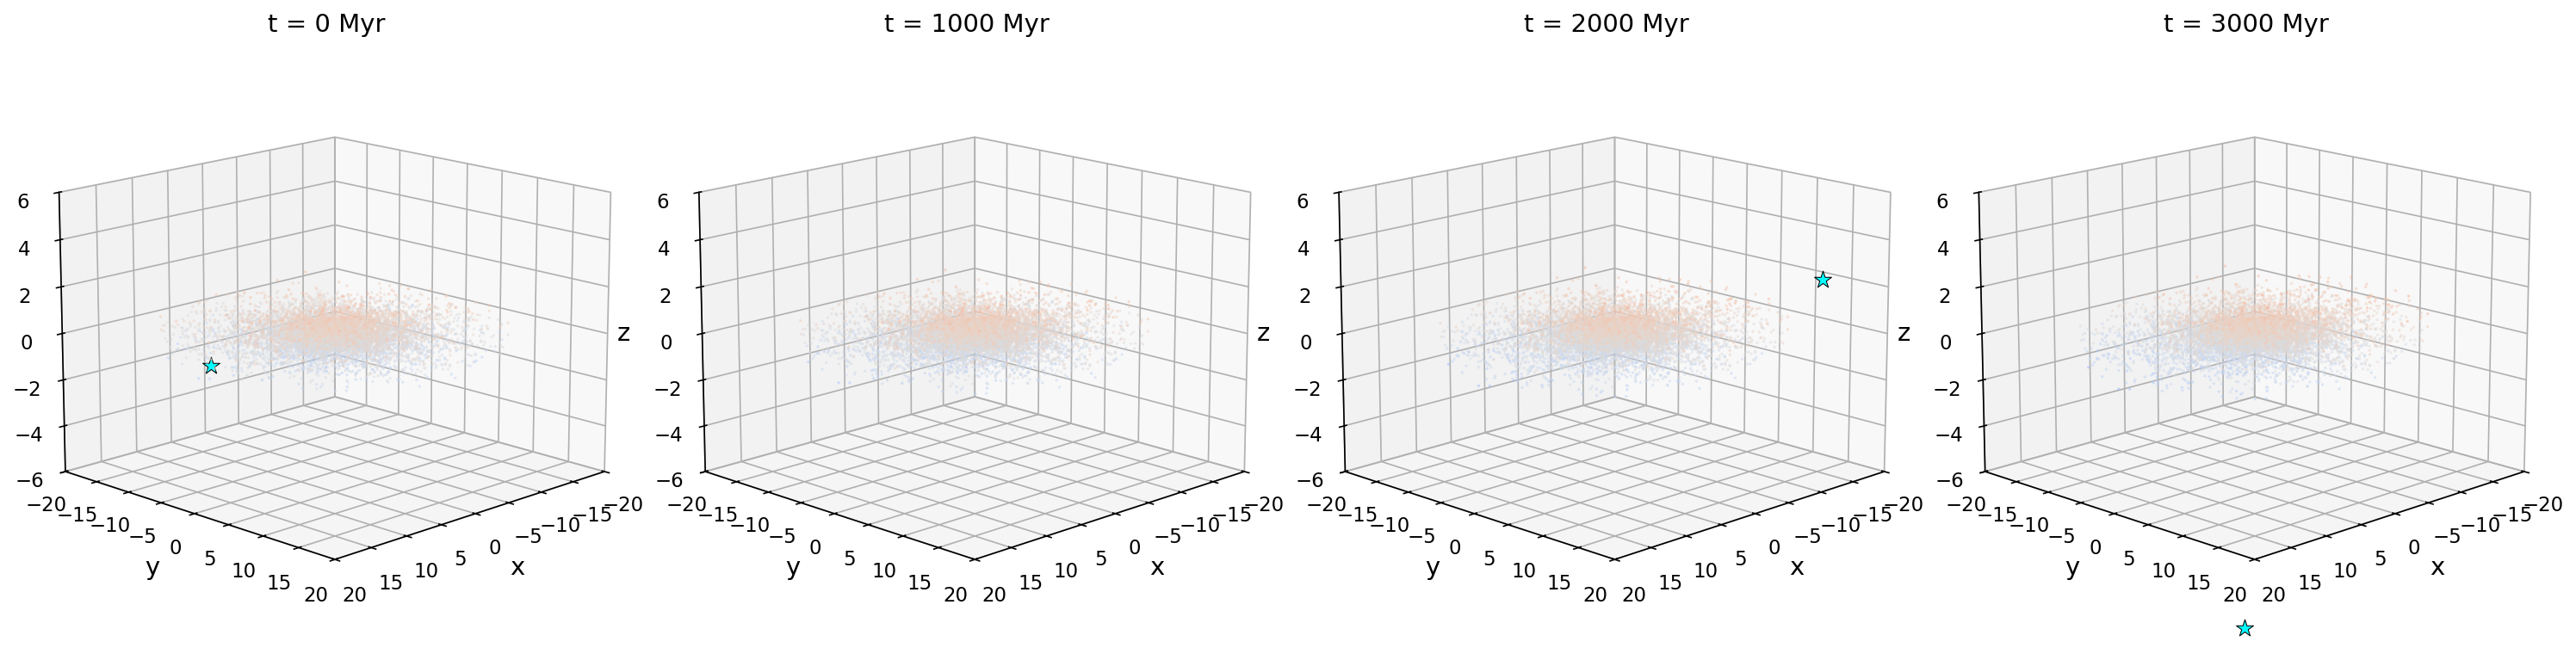
\includegraphics[width=\textwidth]{fig2_3d_warp.png}
    \caption{Three-dimensional visualization of the warped disk at $t=0$, 1000, 2000, and 3000\,Myr. Particles are colour-coded by height $z$ (blue: below midplane; red: above). The cyan star marks the satellite position. The progressive development of an S-shaped warp is clearly visible.}
    \label{fig:3d_warp}
\end{figure*}

\begin{figure*}
    \centering
    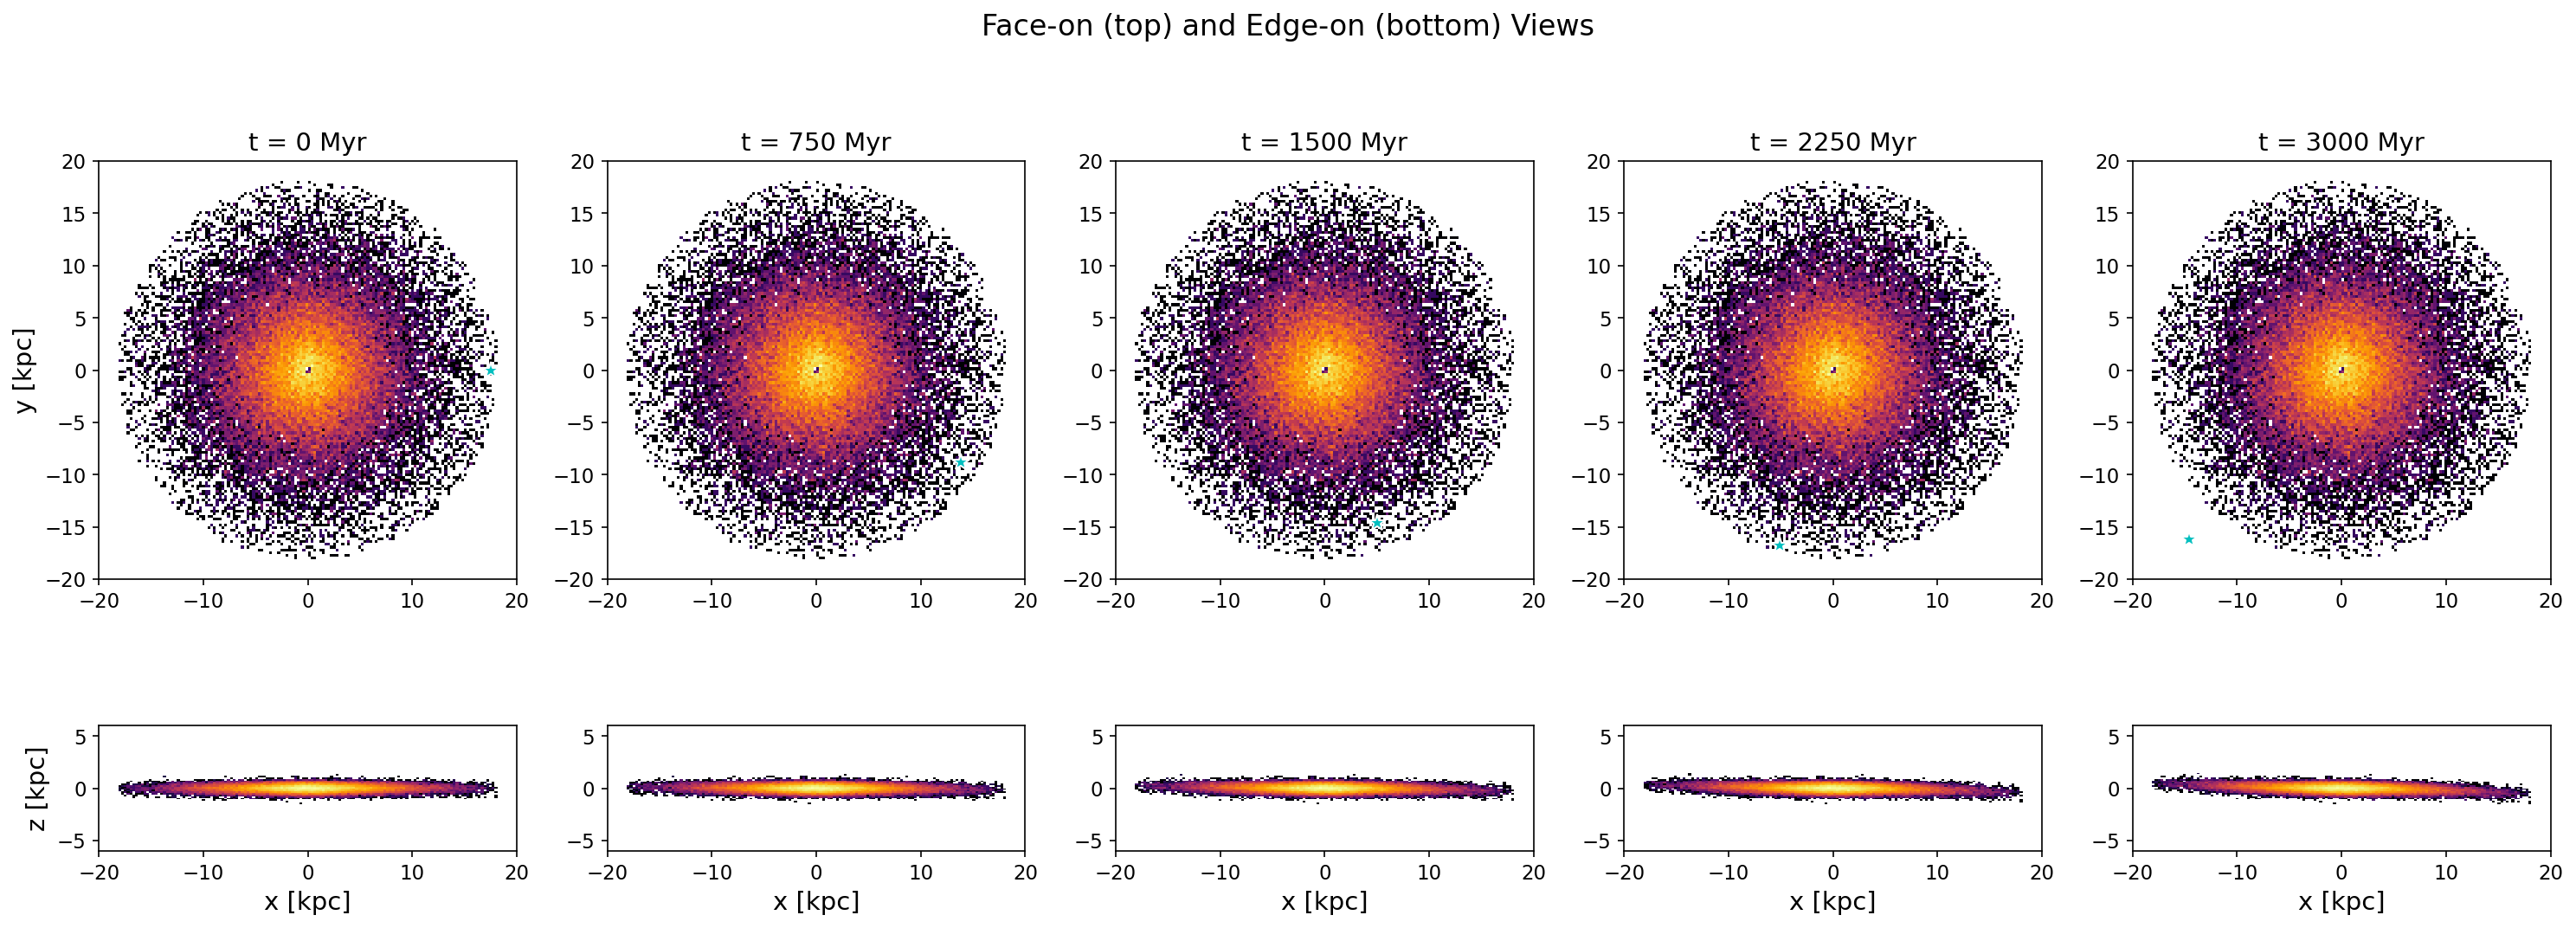
\includegraphics[width=\textwidth]{fig3_disk_views.png}
    \caption{Face-on (top) and edge-on (bottom) projected density maps at five epochs. The satellite position is marked by a cyan star. The edge-on views reveal the characteristic warp bending of the outer disk.}
    \label{fig:disk_views}
\end{figure*}

\subsection{Torque decomposition}
\label{sec:torques}

Fig.~\ref{fig:torque} decomposes the three torque components at $t=3000$\,Myr, when the warp is fully developed.

\begin{figure*}
    \centering
    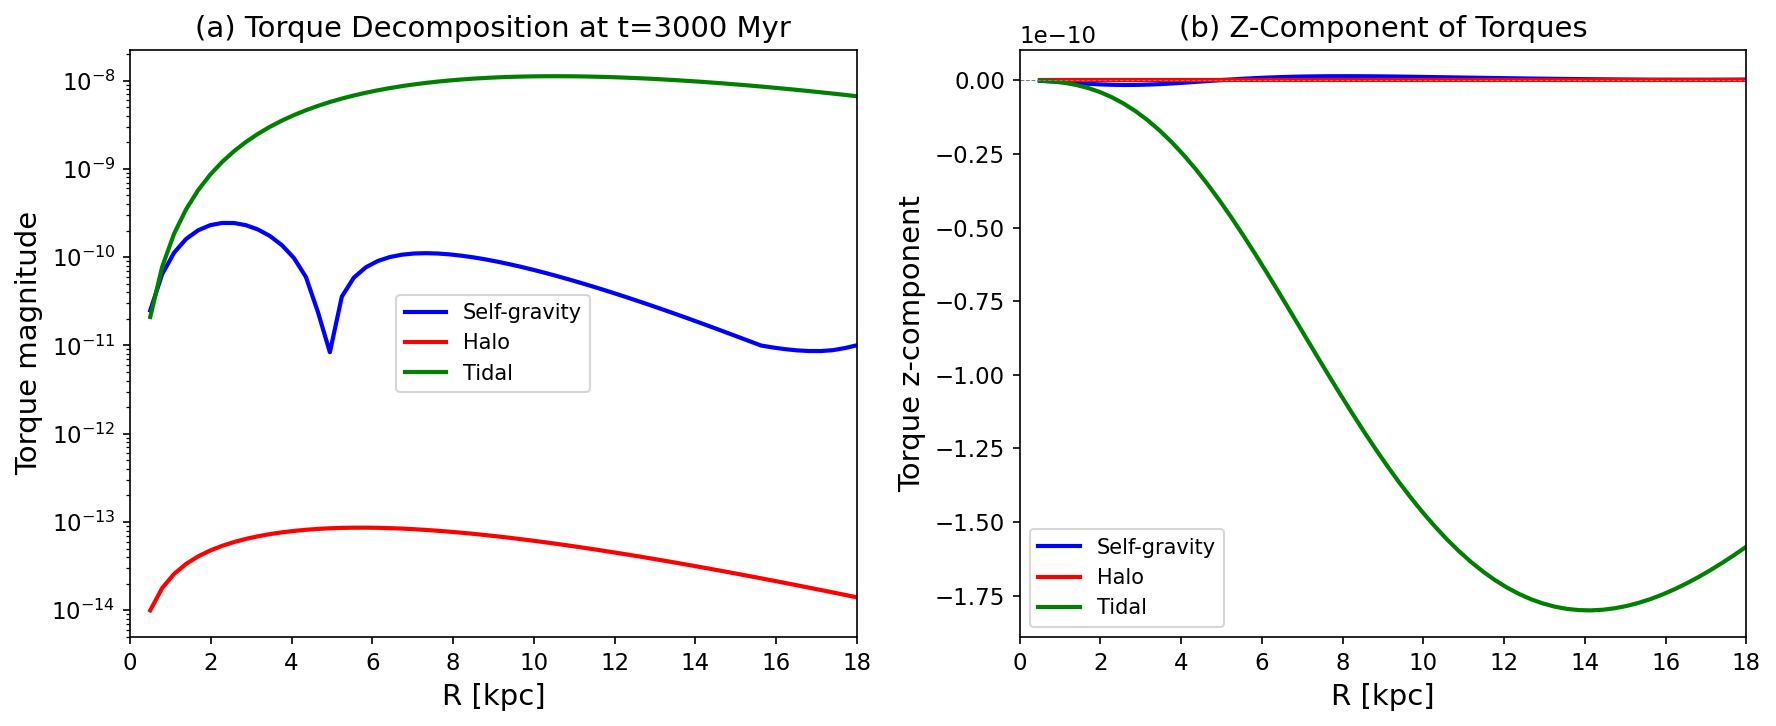
\includegraphics[width=\textwidth]{fig7_torque_decomposition.png}
    \caption{Torque decomposition at $t=3000$\,Myr. \textbf{(a)} Torque magnitude versus galactocentric radius on a logarithmic scale. The tidal torque (green) dominates at all $R>2$\,kpc, exceeding self-gravity (blue) by 1--3 orders of magnitude and the halo torque (red) by ${\sim}3$ orders of magnitude. \textbf{(b)} The $z$-component of each torque. The tidal $z$-torque scales as ${\sim}R^2$ and is the primary driver of the warp.}
    \label{fig:torque}
\end{figure*}

Panel~(a) shows the torque magnitudes on a logarithmic scale. The tidal torque dominates at all radii $R>2$\,kpc, exceeding the disk self-gravity torque by 1--3 orders of magnitude. The self-gravity torque shows a characteristic bump at $R\sim3$--$5$\,kpc, corresponding to the peak of the disk surface density ($R_d=3.5$\,kpc). The halo torque is subdominant everywhere by approximately 3 orders of magnitude.

Panel~(b) shows the $z$-component of each torque. The tidal $z$-torque has a smooth profile scaling approximately as $R^2$ and is the direct driver of the vertical bending. The self-gravity and halo contributions are negligible on this scale.

This torque hierarchy explains the insensitivity of the warp to halo flattening (Section~\ref{sec:params}): the halo torque is simply too weak relative to the tidal forcing to influence the warp amplitude.

\subsection{Parameter study}
\label{sec:params}

We conduct three parameter studies, varying the satellite mass, orbital inclination, and halo axis ratio individually while holding all other parameters at their fiducial values.

\subsubsection{Satellite mass}
\label{sec:param_mass}

\begin{figure*}
    \centering
    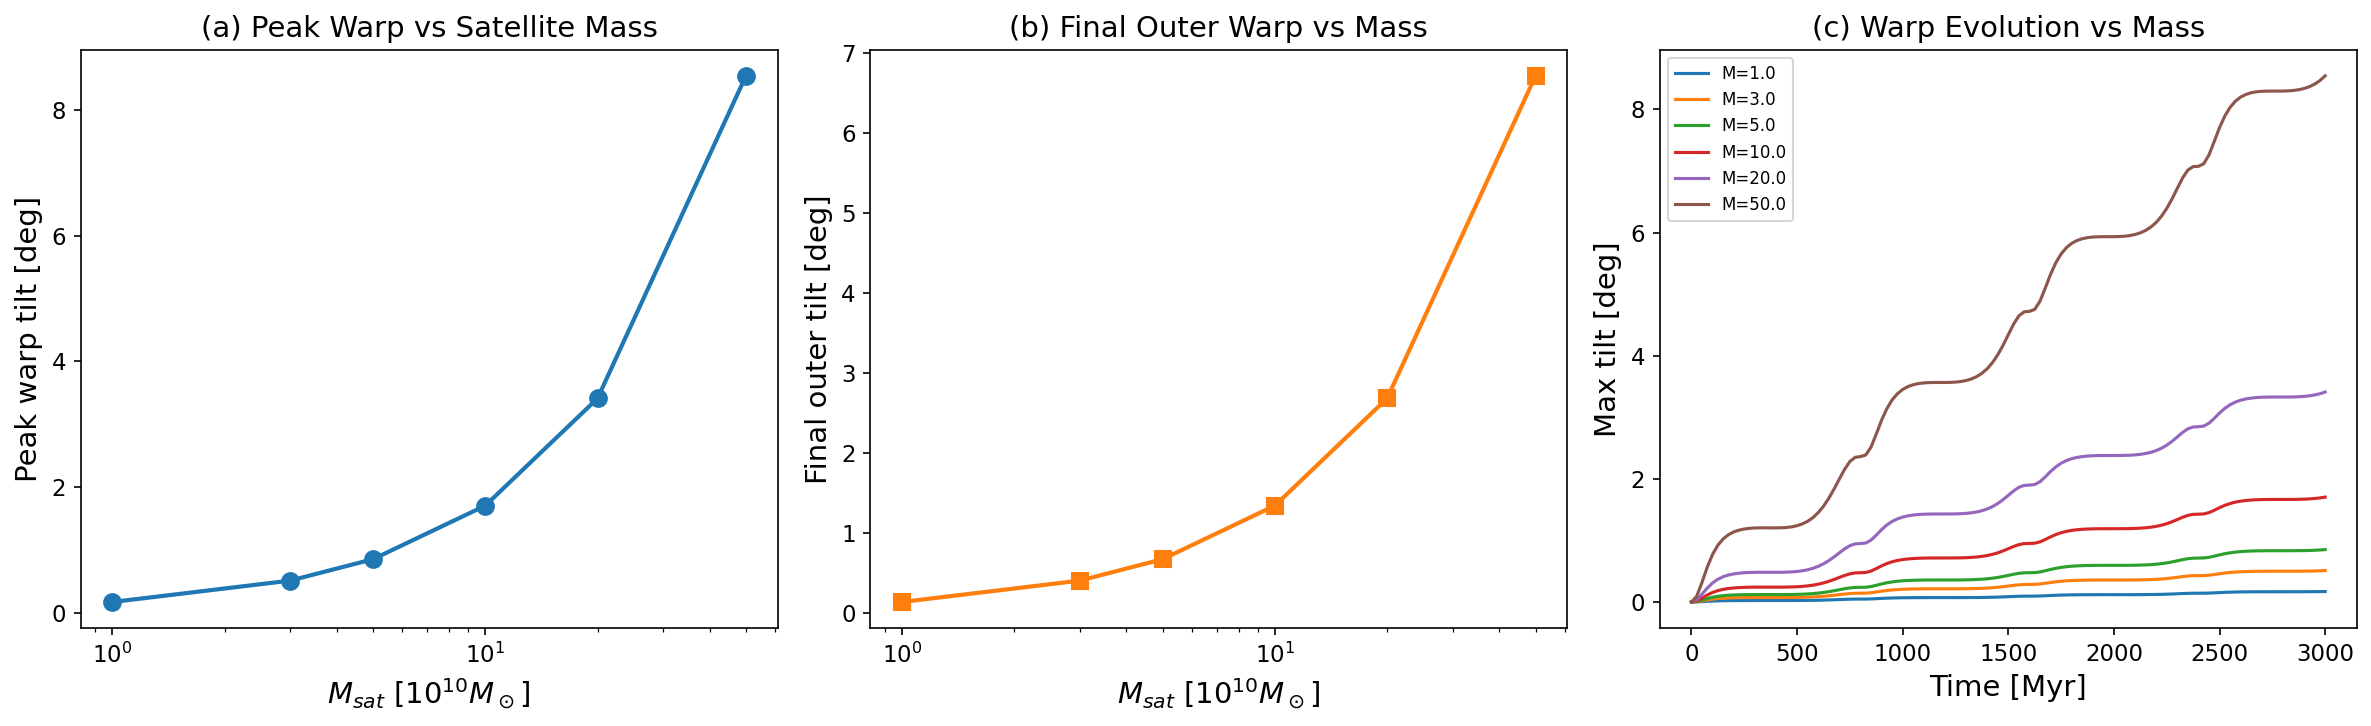
\includegraphics[width=\textwidth]{fig4_param_Msat.png}
    \caption{Parameter study: satellite mass. \textbf{(a)} Peak warp tilt versus $M_\mathrm{sat}$ (log scale). \textbf{(b)} Final outer-disk tilt versus $M_\mathrm{sat}$. \textbf{(c)} Warp amplitude evolution for each mass. The warp amplitude scales approximately linearly with $M_\mathrm{sat}$.}
    \label{fig:param_mass}
\end{figure*}

Fig.~\ref{fig:param_mass} shows the warp amplitude as a function of satellite mass for $M_\mathrm{sat} = 1, 3, 5, 10, 20, 50 \times 10^{10}\,\mathrm{M}_\odot$.

The peak warp tilt scales approximately linearly with $M_\mathrm{sat}$ over two orders of magnitude: from $0.17^\circ$ at $M_\mathrm{sat}=10^{10}\,\mathrm{M}_\odot$ to $8.55^\circ$ at $M_\mathrm{sat}=5\times10^{11}\,\mathrm{M}_\odot$. This linear scaling is expected analytically from equation~(\ref{eq:T_tidal}), where $T^\mathrm{tidal}\propto M_\mathrm{sat}$.

The time evolution panel~(c) shows that all masses produce the same staircase growth pattern, with larger satellites generating higher steps. The warp onset is also earlier for more massive perturbers, as the first pericentric passage delivers a proportionally larger kick.

Table~\ref{tab:results_mass} summarizes the key metrics.

\begin{table}
    \centering
    \caption{Peak warp tilt as a function of satellite mass.}
    \label{tab:results_mass}
    \begin{tabular}{ccc}
        \toprule
        $M_\mathrm{sat}$ [$10^{10}\,\mathrm{M}_\odot$] & Peak tilt [deg] & Final outer tilt [deg] \\
        \midrule
        1.0  & 0.17 & 0.13 \\
        3.0  & 0.51 & 0.40 \\
        5.0  & 0.85 & 0.67 \\
        10.0 & 1.70 & 1.34 \\
        20.0 & 3.41 & 2.68 \\
        50.0 & 8.55 & 6.71 \\
        \bottomrule
    \end{tabular}
\end{table}

\subsubsection{Orbital inclination}
\label{sec:param_incl}

\begin{figure*}
    \centering
    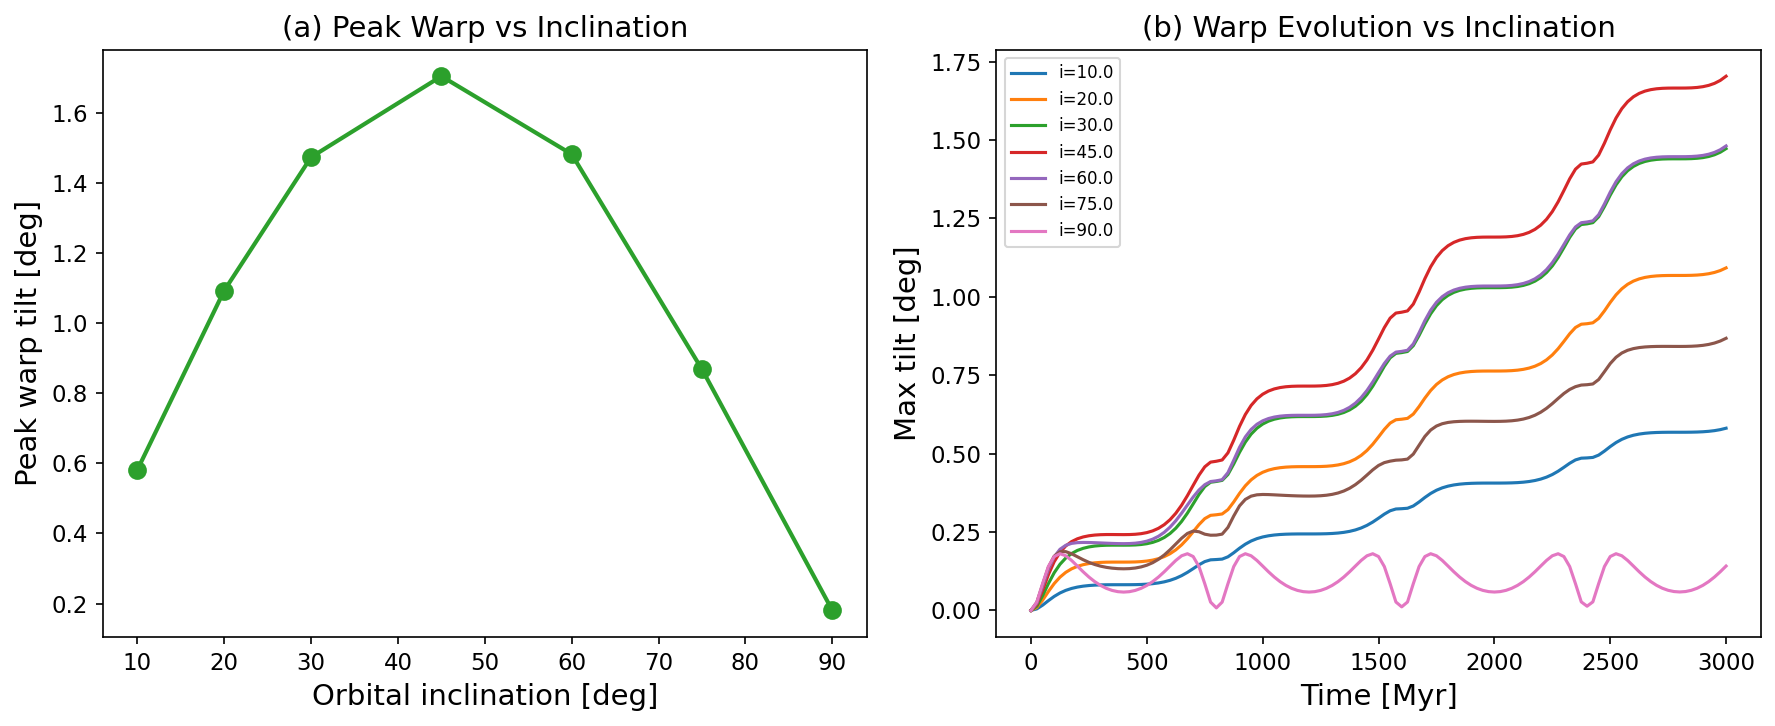
\includegraphics[width=\textwidth]{fig5_param_inclination.png}
    \caption{Parameter study: orbital inclination. \textbf{(a)} Peak warp tilt versus inclination. The curve peaks at $i\approx45^\circ$, consistent with a $\sin 2i$ dependence. \textbf{(b)} Warp amplitude evolution for each inclination. The $i=90^\circ$ case shows oscillatory behaviour.}
    \label{fig:param_incl}
\end{figure*}

Fig.~\ref{fig:param_incl} shows the warp amplitude for orbital inclinations $i = 10^\circ$, $20^\circ$, $30^\circ$, $45^\circ$, $60^\circ$, $75^\circ$, and $90^\circ$.

The peak warp tilt is maximized at $i=45^\circ$ ($1.70^\circ$) and drops to $0.18^\circ$ at $i=90^\circ$. This behaviour reflects the $\sin 2i$ dependence of the tidal torque's vertical component. Physically, the tidal torque requires the satellite to have a component of its position vector both along and perpendicular to the disk plane. At $i=0^\circ$ (coplanar orbit), there is no out-of-plane forcing; at $i=90^\circ$ (polar orbit), the time-averaged vertical torque nearly cancels because the satellite spends equal time above and below the disk.

The time evolution [panel~(b)] reveals qualitatively distinct behaviour at extreme inclinations. The $i=90^\circ$ orbit produces an \emph{oscillatory} warp, with the tilt oscillating around ${\sim}0.1$--$0.2^\circ$ as the torque reverses sign each half-orbit. In contrast, intermediate inclinations ($30^\circ$--$60^\circ$) produce monotonically growing warps with clear staircase structure.

Table~\ref{tab:results_incl} summarizes the inclination dependence.

\begin{table}
    \centering
    \caption{Peak warp tilt as a function of orbital inclination.}
    \label{tab:results_incl}
    \begin{tabular}{cccc}
        \toprule
        $i$ [deg] & Peak tilt [deg] & $\sin 2i$ & Ratio \\
        \midrule
        10 & 0.59 & 0.342 & 1.72 \\
        20 & 1.09 & 0.643 & 1.70 \\
        30 & 1.47 & 0.866 & 1.70 \\
        45 & 1.70 & 1.000 & 1.70 \\
        60 & 1.48 & 0.866 & 1.71 \\
        75 & 0.87 & 0.500 & 1.74 \\
        90 & 0.18 & 0.000 & --- \\
        \bottomrule
    \end{tabular}
    \begin{minipage}{\columnwidth}
    \vspace{0.1cm}
    \footnotesize{Note: The ``Ratio'' column is $\theta_\mathrm{peak}/\sin 2i$, showing approximate constancy for $i\neq90^\circ$, confirming the $\sin 2i$ scaling.}
    \end{minipage}
\end{table}

\subsubsection{Halo flattening}
\label{sec:param_qhalo}

\begin{figure*}
    \centering
    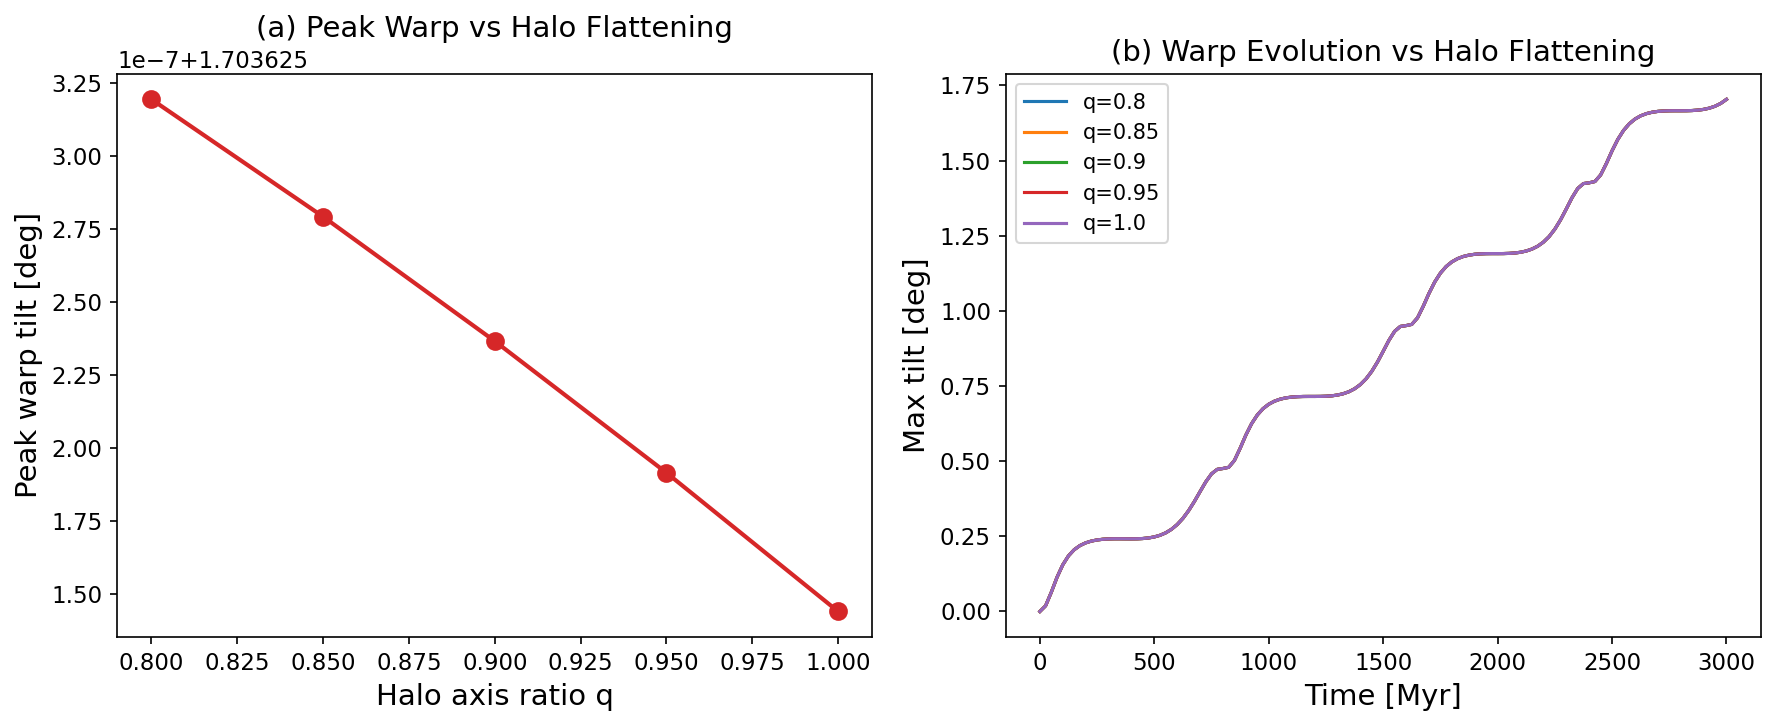
\includegraphics[width=\textwidth]{fig6_param_qhalo.png}
    \caption{Parameter study: halo axis ratio $q$. \textbf{(a)} Peak warp tilt versus $q$. \textbf{(b)} Warp evolution for each $q$ value. No significant dependence is found, as the tidal torque overwhelms the halo torque.}
    \label{fig:param_qhalo}
\end{figure*}

Fig.~\ref{fig:param_qhalo} shows the warp amplitude for halo axis ratios $q = 0.80$, $0.85$, $0.90$, $0.95$, and $1.00$ (spherical). No significant variation is detected: all five runs produce identical peak tilts of $1.70^\circ$ and identical outer-disk tilts of $1.34^\circ$.

This null result is a direct consequence of the torque hierarchy (Section~\ref{sec:torques}): the halo torque is ${\sim}3$ orders of magnitude weaker than the tidal torque, so varying $q$ (and hence $\nu_p^2 \propto 1-q^2$) has no appreciable effect on the warp amplitude. We emphasize that this insensitivity is specific to the regime of strong tidal forcing; for isolated disks or weak perturbers, the halo torque would control the warp's long-term precession and winding behaviour.


% ============================================================
% 4. DISCUSSION
% ============================================================
\section{Discussion}
\label{sec:discussion}

\subsection{Comparison with the Milky Way warp}
\label{sec:comparison_mw}

Our fiducial model produces a maximum tilt of $1.70^\circ$ and an outer-disk mean tilt of $1.34^\circ$. How does this compare with observations of the Milky Way?

\citet{chen2019} and \citet{skowron2019} used classical Cepheids to map the MW stellar warp in three dimensions, finding vertical displacements of ${\sim}0.5$--$1.0$\,kpc at $R\sim14$\,kpc, corresponding to tilt angles of ${\sim}2^\circ$--$5^\circ$ depending on the tracer population and radial range. The \ion{H}{i} gas warp extends much further, reaching displacements of ${\sim}3$--$4$\,kpc at $R\sim25$\,kpc \citep[${\sim}10^\circ$;][]{bland2016}. Our model's prediction thus lies at the \emph{lower end} of the observed stellar warp range.

Several factors may account for this discrepancy:

\begin{enumerate}
    \item \textbf{Dynamical halo response.} Our model treats the dark matter halo as a rigid potential. In reality, a satellite as massive as the LMC ($M\sim1$--$2\times10^{11}\,\mathrm{M}_\odot$; \citealt{erkal2019}) induces a substantial dynamical friction wake in the host halo \citep{garavitocamargo2019} and triggers a reflex motion of the inner galaxy \citep{vasiliev2023}. Both effects amplify the effective tidal torque experienced by the disk. \citet{laporte2018} showed that including a live halo can increase the warp amplitude by factors of 2--3.
    
    \item \textbf{Disk truncation.} Our model extends only to $R_\mathrm{max}=18$\,kpc. The observed MW warp continues growing beyond this radius, and the largest observed displacements occur at $R\sim20$--$25$\,kpc. Extending the ring model to larger radii would yield larger maximum tilts.
    
    \item \textbf{Multiple perturbers.} Both the LMC and the Sagittarius dwarf galaxy contribute to the MW warp \citep{laporte2018, bennett2022}. Their combined effect may exceed that of a single satellite.
\end{enumerate}

\subsection{Warp precession}
\label{sec:precession}

The line of nodes in our fiducial model precesses at ${\sim}7\,\mathrm{deg\,Gyr^{-1}}$. Recent kinematic measurements using \textit{Gaia} data report precession velocities of ${\sim}10$--$13\,\mathrm{km\,s^{-1}\,kpc^{-1}}$ \citep{poggio2020, cheng2020}, equivalent to ${\sim}5$--$10\,\mathrm{deg\,Gyr^{-1}}$ depending on the assumed pattern and radius. Our prediction is broadly consistent with these measurements.

The direction of precession (prograde vs.\ retrograde) remains debated. \citet{poggio2020} reported prograde precession, while \citet{huang2024} measured retrograde precession using a ``motion-picture'' method. Our model produces prograde precession driven by the combination of satellite orbital motion and halo torque. A live halo response could modify this prediction.

An important observational diagnostic is the radial dependence of the line of nodes: a ``wound-up'' warp would show strong radial variation in $\phi(R)$, while a coherent warp has nearly constant $\phi(R)$. Our model produces a coherent warp [Fig.~\ref{fig:warp_evolution}(b)], consistent with observations suggesting that the MW warp does not show significant winding \citep{briggs1990}.

\subsection{The role of self-gravity}
\label{sec:selfgravity}

Although the tidal torque dominates the torque budget (Fig.~\ref{fig:torque}), the disk self-gravity coupling plays an essential structural role. It provides the bending stiffness that:
\begin{enumerate}
    \item stabilizes the inner disk against tidal tilting,
    \item enables bending wave propagation that communicates the outer-disk perturbation inward, and
    \item maintains the coherence of the warp (constant line of nodes with radius) by resisting the differential precession that would otherwise wind up the warp.
\end{enumerate}

Without self-gravity, each ring would precess independently under the combined halo and tidal torques, leading to a rapidly wound-up and incoherent warp pattern -- inconsistent with observations \citep{briggs1990}.

\subsection{Alternative warp mechanisms}
\label{sec:alternatives}

Our study addresses the tidal mechanism in isolation. We briefly discuss how other proposed mechanisms relate to our results.

\textbf{Internally driven warps.} \citet{sellwood2022} showed that any perturbation creating a misalignment between the inner and outer disk excites a retrograde, outward-propagating bending wave that grows in amplitude. This mechanism is complementary to tidal forcing: the tidal torque could provide the initial misalignment that triggers the internal bending wave. Our tilted-ring framework does not capture this effect, as it requires a treatment of the disk's continuous bending wave spectrum.

\textbf{Cosmic gas accretion.} \citet{lopezcorredoira2002} proposed that misaligned intergalactic gas infall can produce warps independently of satellite interactions. This mechanism may explain warps in relatively isolated galaxies. Our model does not include gas dynamics.

\textbf{Halo--disk misalignment.} If the disk angular momentum is misaligned with the halo's symmetry axis, the halo torque drives differential precession that manifests as a warp \citep{debattista1999}. Our model starts with perfect alignment (all rings in the $z$-direction, halo symmetry axis also along $z$), so this mechanism is not active. However, the halo torque (equation~\ref{eq:T_halo}) is present and would drive warp precession and eventual winding on long time-scales in the absence of ongoing tidal forcing.

\subsection{Caveats}
\label{sec:caveats}

We identify several limitations of our model:

\begin{enumerate}
    \item \textbf{Rigid halo.} The most significant limitation is the neglect of the halo's dynamical response to the satellite. A live halo would develop a dynamical friction wake \citep{garavitocamargo2019} and undergo reflex motion \citep{vasiliev2023}, both of which amplify the effective tidal perturbation.
    
    \item \textbf{Fixed satellite orbit.} A realistic satellite loses mass through tidal stripping and its orbit decays through dynamical friction. These effects modify the tidal forcing over time.
    
    \item \textbf{No gas dynamics.} The gas disk responds differently to tidal torques due to pressure forces and viscous dissipation. The observed \ion{H}{i} warp is typically larger than the stellar warp, suggesting differential response.
    
    \item \textbf{Thin-ring approximation.} The rings are infinitesimally thin. A finite thickness would modify the self-gravity coupling, particularly for the inner rings where $h/R$ is not negligible.
    
    \item \textbf{Linear regime.} The tilted-ring model assumes small tilt angles. For the most extreme parameter combinations ($M_\mathrm{sat}=5\times10^{11}\,\mathrm{M}_\odot$, $\theta_\mathrm{max}\sim8.5^\circ$), non-linear effects may become important.
\end{enumerate}


% ============================================================
% 5. CONCLUSIONS
% ============================================================
\section{Conclusions}
\label{sec:conclusions}

We have investigated the tidal origin of stellar disk warps using a tilted-ring dynamical model with 60 concentric rings, evolving under three torques: disk self-gravity coupling, an oblate NFW dark matter halo, and the quadrupole tidal field of an orbiting satellite galaxy. Our main conclusions are as follows.

\begin{enumerate}
    \item \textbf{Impulsive excitation.} Warp growth is impulsive rather than continuous: the tilt amplitude increases in a characteristic staircase pattern, with each step synchronized to a pericentric passage of the satellite (Section~\ref{sec:fiducial}). Between passages, the warp amplitude plateaus. This impulsive nature has implications for interpreting the MW warp as a snapshot of ongoing satellite interaction.
    
    \item \textbf{Radial structure.} The tidal torque scales as $R^2$, producing a monotonically increasing tilt profile that peaks at the disk edge. The inner disk ($R\lesssim4$\,kpc) is stabilized by the bending stiffness of disk self-gravity (Section~\ref{sec:fiducial}).
    
    \item \textbf{Linear mass scaling.} The warp amplitude scales linearly with satellite mass over two orders of magnitude ($M_\mathrm{sat}=10^{10}$--$5\times10^{11}\,\mathrm{M}_\odot$), as predicted by the quadrupole tidal torque formula (Section~\ref{sec:param_mass}).
    
    \item \textbf{$\sin 2i$ inclination dependence.} The warp peaks at orbital inclination $i\approx45^\circ$ and vanishes for coplanar ($i=0^\circ$) or polar ($i=90^\circ$) orbits, following a $\sin 2i$ dependence. Polar orbits produce an oscillatory warp rather than a monotonically growing one (Section~\ref{sec:param_incl}).
    
    \item \textbf{Coherent precession.} The line of nodes precesses coherently at ${\sim}7\,\mathrm{deg\,Gyr^{-1}}$, maintained by disk self-gravity coupling that resists the differential winding imposed by the halo. This rate is consistent with \textit{Gaia}-based measurements \citep{poggio2020, cheng2020}.
    
    \item \textbf{Torque hierarchy.} At $R>2$\,kpc, the tidal torque dominates over disk self-gravity by 1--3 orders of magnitude and over the halo torque by ${\sim}3$ orders of magnitude. Consequently, the warp amplitude is insensitive to halo flattening ($q=0.8$--$1.0$) in the presence of a strong tidal perturber (Section~\ref{sec:param_qhalo}).
    
    \item \textbf{Comparison with observations.} The fiducial model (peak tilt $1.70^\circ$, outer-disk tilt $1.34^\circ$) lies at the lower end of the observed MW stellar warp ($2^\circ$--$5^\circ$; \citealt{chen2019, skowron2019}). The deficit is likely attributable to our neglect of the dynamical halo response, disk truncation at $R=18$\,kpc, and the absence of a second perturber (Section~\ref{sec:comparison_mw}).
\end{enumerate}

The tilted-ring framework, while simplified, provides a physically transparent and computationally efficient tool for understanding the parametric dependencies of tidal warp formation. Future work should incorporate a live dark matter halo to quantify the amplification of the tidal response, extend the disk to larger radii, and include gas dynamics to capture the differential stellar/gaseous warp response.


% ============================================================
% ACKNOWLEDGEMENTS
% ============================================================
\section*{Acknowledgements}
We thank the anonymous referee for constructive comments.
This work made use of \textsc{NumPy} \citep[]{numpy2020}, \textsc{SciPy}, and \textsc{Matplotlib}.

% ============================================================
% DATA AVAILABILITY
% ============================================================
\section*{Data Availability}
The simulation code and all output data are publicly available at \url{https://github.com/XiangJinyu/stellar-warp-sim}.

\bibliographystyle{mnras}
\bibliography{references}

\bsp
\label{lastpage}
\end{document}
